% Plan de la présentation
\section*{Plan}

\begin{frame}{Plan de la présentation}
    \begin{center}
        \begin{minipage}{0.9\textwidth}
            \tableofcontents[hideallsubsections]
        \end{minipage}
    \end{center}
\end{frame}

% Définition des sections pour la table des matières
\section{Introduction}
\begin{frame}{}
    \sectionpage
    \begin{center}
        \Large\textbf{Introduction}
        \vspace{1cm}
        
        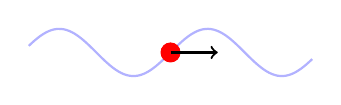
\begin{tikzpicture}[scale=0.6]
            % Représentation simple d'une particule et son champ d'onde
            \draw[thick, blue!30, smooth] plot[domain=-3:3,samples=50] 
                (\x,{0.5*sin(2*\x r)});
            \filldraw[red] (0,0) circle (0.2);
            \draw[->,thick] (0,0) -- (1,0);
        \end{tikzpicture}
    \end{center}
\end{frame}

% \section{Modèle mathématique}
% \section{Approche initiale : RK4 séquentiel}
% \section{Tentative de parallélisation avec MPI}
% \section{L'algorithme Parareal}
% \section{Implémentation}
% \section{Résultats}
% \section{Discussion et Conclusion}

% % Définition des sous-sections si nécessaire
% \subsection{Contexte physique}
% \subsection{Équations du système}
% \subsection{Objectifs de parallélisation}